\cleardoublepage

\part{Versuche}\label{part:Exercises}
	\thispagestyle{empty}
	\cleardoublepage
	
	\chapter{Sender}\label{chap:sender}
	\thispagestyle{empty}

	\begin{figure}
		\centering 
		%\psfrag{01}{MATLAB Workspace}
		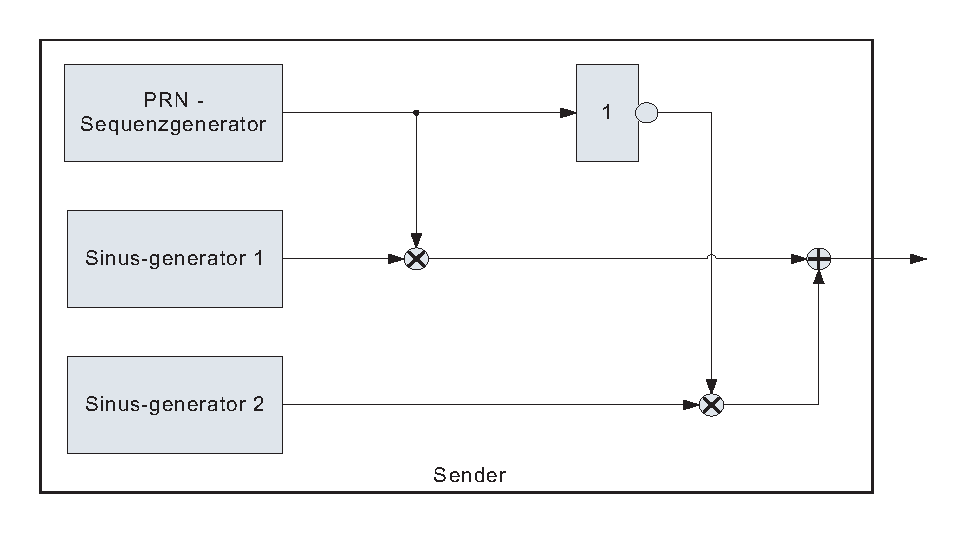
\includegraphics[width=10cm]{bilder/sender/sender_blockschaltbild}
		\caption{Sender Blockschaltbild}
		\label{abb:sender_blockschaltbild}
		\index{Sender Blockschaltbild}
	\end{figure}

Mittels des in Abb. \ref{abb:sender_blockschaltbild} dargestellten Systems werden die zu �bertragenden Signale erzeugt. Es besteht aus einem Pseudo-Zufallszahlen-Generator, dessen Ausgangssignal mit Hilfe eines einfachen FSK-Modulators moduliert werden soll. Eine detailliertere Beschreibung der einzelnen Komponenten wird in den folgenden Kapiteln erarbeitet.